\documentclass{article}
\usepackage[utf8]{inputenc}
\usepackage[brazil]{babel}
\usepackage{url}
\usepackage{tabularx}
\usepackage{palatino}
\usepackage{hyperref}
\usepackage{pdfpages}
\usepackage[margin=2.5cm]{geometry}

\title{\textbf{MAC0213 - Atividade Curricular em Comunidade \\ Projeto 5: Desenvolvimento de análises de dados históricos}}
\author{
	Uma parceria \textit{Tecs: grupo de comput\{ação social\} da USP} \\ e \textit{Secretaria Municipal de Educação} \\
    \\
    \textbf{Aluno:} Luís Felipe de Melo  \\
    \textbf{Número USP:} 9297961
    }
\date{}

\begin{document}
\maketitle

\section{Introdução}

Instituída pela Portaria nº 3.786, de 17 de abril de 2017, da Secretaria Municipal de Educação (SME), a Política de Governo Aberto “Pátio Digital” tem como objetivo aproximar diferentes setores da sociedade para promover ações de abertura de dados, metodologias colaborativas e inovação tecnológica na gestão da Rede Municipal de Educação e na entrega de serviços educacionais à população.

O Pátio Digital está estruturado em três eixos: 

\begin{enumerate}
\item “Transparência e Dados Abertos”, com o fortalecimento da disponibilização de dados públicos e informações sobre as políticas educacionais;
\item “Inovação Tecnológica”, com a construção colaborativa de ferramentas e serviços digitais à comunidade escolar, no formato de código aberto;
\item “Colaboração Governo-Sociedade”, que são espaços e metodologias de interação entre o setor público, Academia, sociedade civil e iniciativa privada.
\end{enumerate}

Dentro deste último eixo, “Colaboração Governo-Sociedade”, se insere o Programa de Cooperação em Pesquisa, que tem como objetivo conectar a Secretaria Municipal de Educação com o campo acadêmico, estabelecendo mecanismos para o desenvolvimento de projetos e ações que estimulem a produção de conhecimento sobre as políticas educacionais do município. 

É no âmbito do Programa de Cooperação em Pesquisa que se estabelece a colaboração entre SME, via Pátio Digital, e \textit{Tecs}, grupo de extensão universitária do Instituto de Matemática e Estatística da USP (IME-USP). A partir do diálogo entre as equipes do Pátio Digital e do Tecs, foram levantados quatro projetos que articulam os conhecimentos da Ciência da Computação e os desafios de políticas públicas educacionais do município. 

\section{A Instituição}

A Secretaria Municipal de Educação é o órgão da Prefeitura Municipal de São Paulo responsável pela oferta de educação infantil em creches e pré-escolas e, em conjunto com o esfera estadual, Ensino Fundamental, Médio e Educação de Jovens e Adultos (EJA). Em sua estrutura, a SME conta com Unidades Educacionais/ Centros Educacionais, Diretorias Regionais de Educação, Órgãos Centrais e o Conselho Municipal de Educação, formando em conjunto a Rede Municipal de Ensino (RME-SP).

Em dezembro de 2017, havia 978.991 alunos em etapas de escolarização na RME-SP, distribuídos em 13 Diretorias Regionais de Educação. 

O Projeto de cooperação se insere no contexto do Pátio Digital, Política de Governo Aberto da SME que propõe a abertura de dados, colaboração com a sociedade e o uso de tecnologias abertas para a melhoria das políticas educacionais. O Comitê Técnico do Pátio Digital é composto por representantes de quatro unidades da SME: Coordenadoria de Transparência Ativa e Controle Interno (COTAC); Coordenadoria de Informações Educacionais (CIEDU); Coordenadoria de Tecnologia da Informação e Comunicação (COTIC); e, por fim, a Assessoria de Comunicação (ASCOM). 

\section{Objetivos}

No Portal de Dados Abertos da Prefeitura de São Paulo, está disponível a série histórica do Microdados Matrículas (2000-2017) e Servidores (2014-2016). Junto com outras bases menores, é possível obter, além de um rico panorama (atual e histórico) sobre a educação municipal, análises aprofundadas sobre diferentes temáticas. 

Ao aderir ao Projeto 5, o aluno deverá identificar cinco temáticas de análises de dados (se possível, alinhadas ao Banco de Desafios do Programa de Cooperação em Pesquisa). Após o desenho do projeto, o aluno desenvolverá, com apoio de áreas internas relacionadas na SME, as análises quantitativas, tais como: 

\begin{itemize}
\item Simulação do tempo de espera na fila da creche;
\item Análises históricas sobre a RME-SP;
\item Análise do perfil dos alunos.
\end{itemize}

Ao aderir a esse projeto, o aluno deverá desenvolver análises extremamente ricas, e que envolvam, além do código e \textit{deliverables} associados, um relatório analítico. 

Serão cinco temáticas de análises de dados alinhadas ao Banco de Desafios do Programa de Cooperação em Pesquisa.


\section{Tarefas}

As atividades terão 100 horas de duração, conforme a divisão a seguir:

\begin{center}
  \begin{tabular}{ | l | l | p{5cm} | l | }
    \hline
    \# & Tópico & Tarefa & Duração prevista \\ \hline
    1 & Apresentação & Desenhar, junto com a supervisora, cronograma do Projeto  & 3 horas \\ \hline
    2 & Identificação & Identificar cinco possíveis análises a partir dos microdados e outras bases já publicadas & 15 horas \\ \hline
    3 & Identificação & Identificar relações com o Banco de Desafios do Programa de Cooperação em Pesquisa & 5 horas \\ \hline
    4 & Participação & Realizar reuniões com áreas internas da SME para alinhamento e eventuais dúvidas & 7 horas \\ \hline
    5 & Resolução & Entregar 3 análises e relatórios técnicos \textbf{até novembro de 2018} & 40 horas  \\ \hline
    6 & Resolução & Entregar 2 análises e relatórios técnicos \textbf{até dezembro de2018} & 30 horas \\ \hline
 \end{tabular}
\end{center}

De maneira geral, para cada uma das cinco análises, as atividades se distribuem em duas horas de reuniões com a Secretaria, duas horas de planejamento e desenho da análise e dezesseis horas de realização da análise, distribuídas entre limpeza, seleção e organização dos dados, escolha do modelo, desenvolvimento do modelo, ajustes finais do modelo, análise dos resultados e escrita do relatório técnico. 

\section{Progresso}

O projeto será acompanhando e monitorado com base no cronograma previamente alinhado entre o aluno e a supervisora. As horas dedicadas ao projeto serão registradas em um \textit{log} que deverá ser assinado pela supervisora e anexado ao relatório final.

Ao final do semestre, como requisito para a conclusão da disciplina, o aluno deverá produzir um relatório final e um pôster sobre as atividades desenvolvidas.

O progresso atual pode ser conferido nesta página: \url{https://lsflp.github.io/MAC0213}.

\section{Supervisora}

O responsável por supervisionar as atividades do aluno  no \textbf{Pátio Digital} será \textbf{Priscilla Corrêa}, cujo e-mail é \texttt{priscilla.santos@sme.prefeitura.sp.gov.br}, \textbf{Assessora Técnica da Secretaria Municipal de Educação de São Paulo}.

Embora o \textit{Tecs} tenha sido responsável por desenvolver o projeto em conjunto com a instituição parceira e disponibilizá-lo a comunidade discente, ele não retém nenhuma responsabilidade quanto ao cumprimento das atividades por parte do aluno. Além disso, a realização do projeto não configura vínculo do aluno com o grupo de extensão.

\section{Carta de Concordância}

A carta de concordância da instituição onde a atividade será realizada está anexa na próxima página.

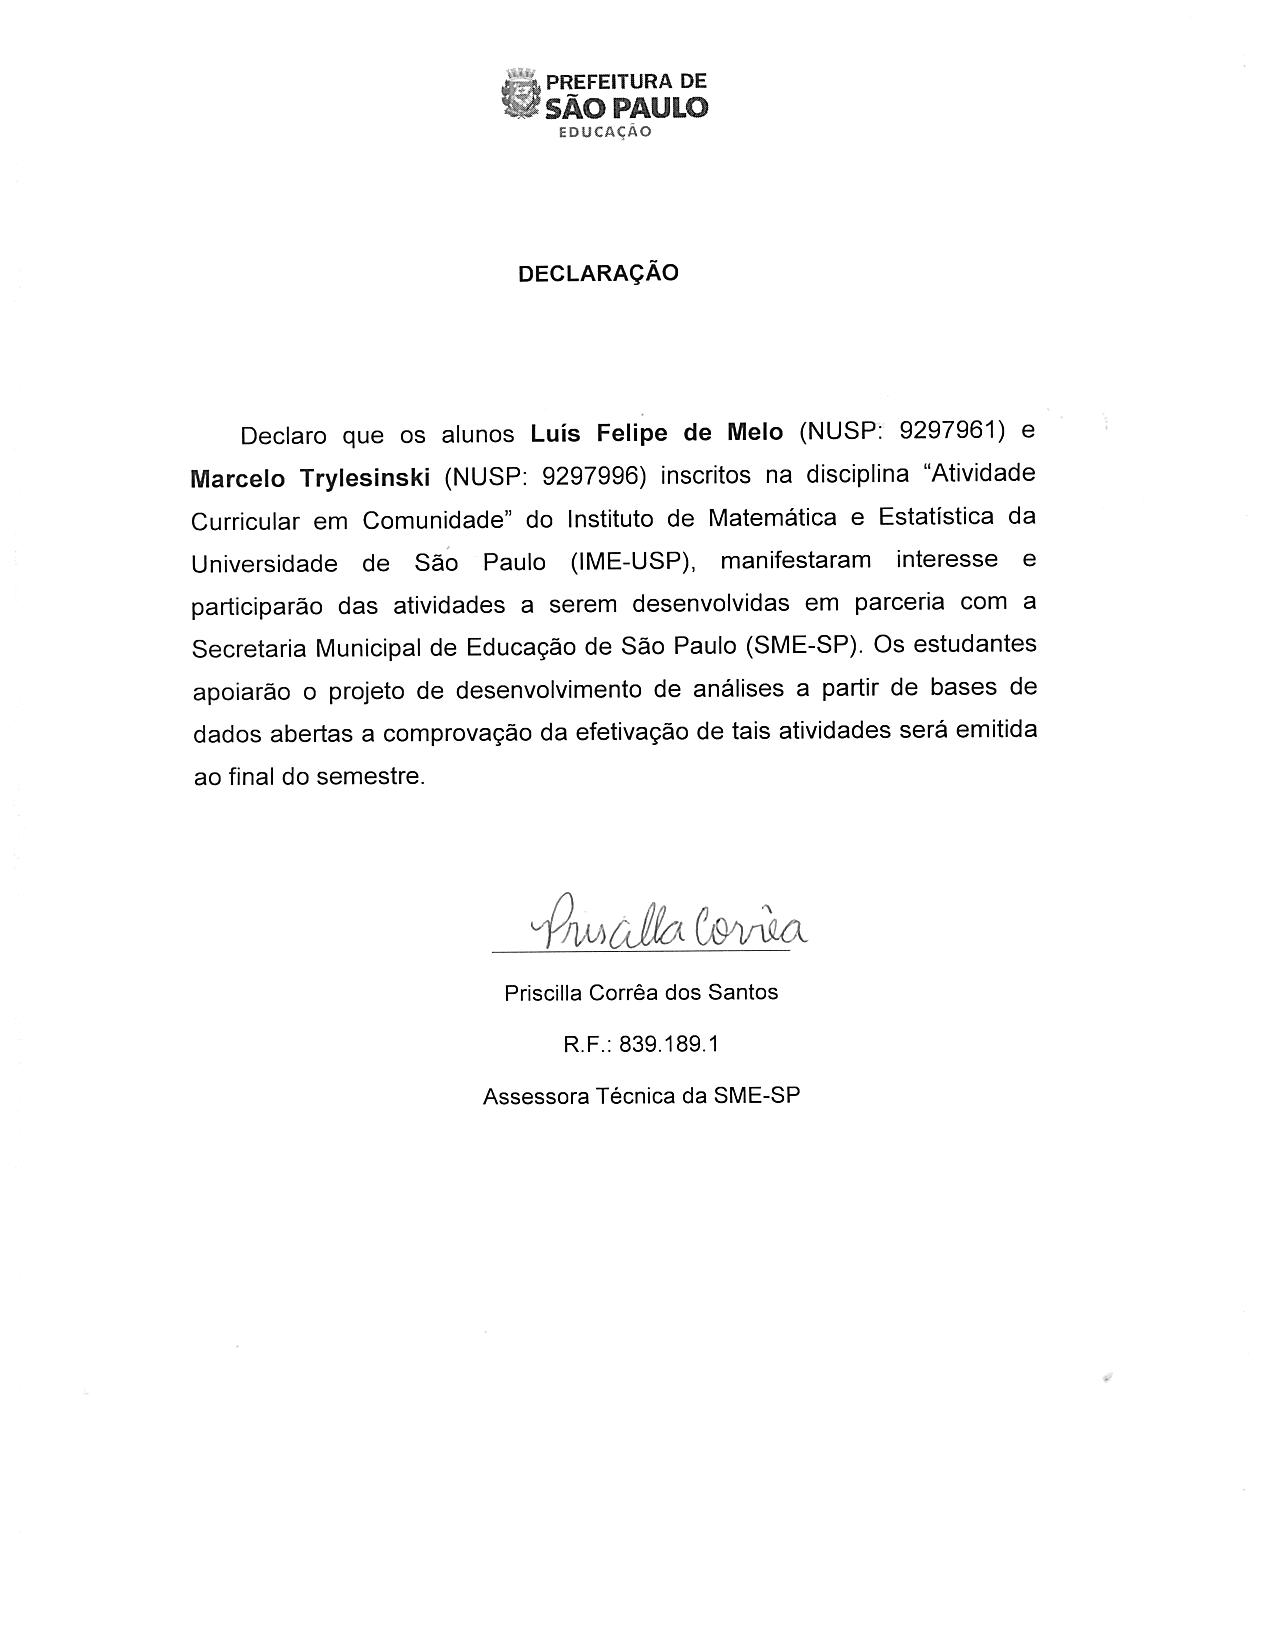
\includepdf{declaracaoanalisedados.pdf}

\end{document}
